%! Mode:: "TeX:UTF-8"
%! TEX program = xelatex
\PassOptionsToPackage{quiet}{xeCJK}
\documentclass[withoutpreface,bwprint]{cumcmthesis}
\usepackage{etoolbox}
\usepackage{ctex}
\BeforeBeginEnvironment{tabular}{\zihao{-5}}
\usepackage[numbers,sort&compress]{natbib}  % 文献管理宏包
\usepackage[framemethod=TikZ]{mdframed}  % 框架宏包
\usepackage{url}  % 网页链接宏包
\usepackage{subcaption}  % 子图宏包
\newcolumntype{C}{>{\centering\arraybackslash}X}
\newcolumntype{R}{>{\raggedleft\arraybackslash}X}
\newcolumntype{L}{>{\raggedright\arraybackslash}X}\renewcommand{\textbf}[1]{{\song\bfseries #1}}

\usepackage{tikz}
\usetikzlibrary{
    shapes.geometric,
    arrows.meta,
    positioning,
    calc,
    angles,
    quotes,
    decorations.markings
}
\tikzstyle{startstop} = [rectangle, rounded corners, minimum width=3cm, minimum height=1cm,text centered, draw=black, fill=red!20]
\tikzstyle{process} = [rectangle, minimum width=3.5cm, minimum height=1cm, text centered, draw=black, fill=blue!20]
\tikzstyle{decision} = [diamond, aspect=2, minimum width=3.5cm, minimum height=1cm, text centered, draw=black, fill=green!20]
\tikzstyle{arrow} = [thick,->,>=stealth]\usetikzlibrary{calc,angles,quotes}
\usepackage{pgfplots}
\pgfplotsset{compat=1.18}
\usepackage{float}

% 机器狗轨迹图颜色
\definecolor{pathgray}{HTML}{3A3F44}
\definecolor{startgreen}{HTML}{2CA02C}
\definecolor{detectblue}{HTML}{1F77B4}
\definecolor{clearred}{HTML}{D62728}
\definecolor{missorange}{HTML}{FF7F0E}
\definecolor{scanpurple}{HTML}{9467BD}























\title{基于集成学习的洪水概率预测}  % 论文标题



%%%%%%%%%%%%%%%%%%%%%%%%%%%%%%%%%%%%%%%%%%%%%%%%%%%%%%%%%%%%%
%% 正文
\begin{document}

% 封面和目录页不显示页码
\pagenumbering{gobble}
\maketitle
\begin{abstract}


\textbf{对于,}

\textbf{对于问题二,}

\textbf{对于问题三,}

\textbf{对于问题四,}

最后，



\keywords{关键词；关键词；关键词；关键词；关键词}

\end{abstract}


%%%%%%%%%%%%%%%%%%%%%%%%%%%%%%%%%%%%%%%%%%%%%%%%%%%%%%%%%%%%% 
%\vspace{-1.4cm} 
%\tableofcontents  % 目录
%\newpage











%%%%%%%%%%%%%%%%%%%%%%%%%%%%%%%%%%%%%%%%%%%%%%%%%%%%%%%%%%%%% 
\pagenumbering{arabic}
\vspace{-1.4cm} 
\section{问题重述}
\subsection{问题背景}

无线电干扰源的快速定位与清除是无线电频谱管理中的重要任务。
现有流程通常包括初步监测、区域排查和精准定位三个阶段，其中精准定位仍主要依赖人工完成，易受环境遮挡、信号强弱及测向误差等因素影响，导致定位与清除效率较低。
为提高任务执行效率，本文考虑利用机器狗搭载无线电测向设备与光学探测设备，实现对干扰源的自动搜索、定位与清除。





%%%%%%%%%%%%%%%%%%%%%%%%%%%%%%%%%%%%%%%%%%%%%%%%%%%%%%%%%%%%% 
\subsection{问题提出}
现已知自动定位清除系统的检测原理和工作方式，以及干扰源的基本信息，本文需要解决以下问题：

\textbf{问题1：}根据监测点位置、示向度及检测误差确定干扰源定位区域，计算其直径，并判断以该直径作圆能否覆盖整个定位区域。

\textbf{问题2：}  根据第一监测点获得的位置与示向信息，确定第二监测点的合理位置，使两次测向形成的交会定位区域尽可能小，以提高定位精度，并便于后续扫描与清除。

\textbf{问题3：} 为机器狗设计自主搜索与决策策略，在全向干扰源总数未知的情况下，确保搜索并清除区域内全部干扰源，同时尽可能缩短任务完成时间，提高整体搜索、定位与清除效率。

\textbf{问题4：}  在问题三的基础上，将部分全向干扰源替换为定向干扰源，且其位置与定向方向均未知。针对定向干扰源信号覆盖范围受限的特点，对原有搜索、定位与清除策略进行调整，在确保所有干扰源均被清除的前提下，尽可能缩短任务完成时间。

















\newpage
%%%%%%%%%%%%%%%%%%%%%%%%%%%%%%%%%%%%%%%%%%%%%%%%%%%%%%%%%%%%% 
\section{问题分析}
\subsection{问题一分析}
问题一中，本文先将每个监测点的坐标、示向度和测向误差转化为直角坐标系中的角域约束，再通过多个角域求交，建立干扰源定位区域的几何模型。随后，将该定位区域表示为多边形，并利用程序枚举顶点对，求出最大顶点距离作为区域直径。最后以该直径构造候选圆，比较多边形各顶点到圆心的距离与圆半径，从而判断该圆能否完全覆盖定位区域。
\subsection{问题二分析}
问题二中，本文结合问题一中交会定位法的结论和机器狗的激光扫描清除方式，将较优扫描区域转化为“定位区域直径较小”且“能够被有效覆盖”两项约束，并据此建立第二监测点选址的几何评价模型。对于平面上的每个候选监测点，统计其能够满足较优检测条件的目标数量，并据此进行评分，从而筛选出最优或较优的第二监测点区域。
\subsection{问题三分析}
问题三需要在实际约束下对机器狗的行为进行决策。在保证所有干扰源均被清除的前提下，同时考虑移动速度、检测时间和清除时间等因素，以最小化总任务时间。为此，本文将总耗时分解为不同任务的时间成本，分别分析其优化空间，并通过合理安排扫描位置、扫描时机和清除顺序，降低整体任务耗时。






















\newpage
%%%%%%%%%%%%%%%%%%%%%%%%%%%%%%%%%%%%%%%%%%%%%%%%%%%%%%%%%%%%% 
\section{模型假设}

为简化问题，本文做出以下假设：

\begin{itemize}[itemindent=2em]
\item 假设1
\item 假设2
\item 假设3
\end{itemize}

%%%%%%%%%%%%%%%%%%%%%%%%%%%%%%%%%%%%%%%%%%%%%%%%%%%%%%%%%%%%% 

\section{符号说明}









\begin{table}[H]
	\centering
	
	\begin{tabularx}{\textwidth}{CL}
		\toprule
		符号    & 说明    \\
		\midrule
		$n$ & 样本总数 \\
		$d$ & 每个样本的特征变量个数 \\
		$\boldsymbol{x}^{(i)}$ & 第 $i$ 个样本的 $d$ 个特征变量，$\boldsymbol{x}^{(i)} = (x_1^{(i)}, x_2^{(i)}, \dots, x_d^{(i)})$ \\
		$y^{(i)}$ & 第 $i$ 个样本对应的洪水发生概率 \\
		$f(\cdot)$ & 构建的预测函数 \\
		$\Omega(f)$ & 正则化项 \\

		\bottomrule
	\end{tabularx}
	
	\label{tab:符号说明}
\end{table}











\newpage
%%%%%%%%%%%%%%%%%%%%%%%%%%%%%%%%%%%%%%%%%%%%%%%%%%%%%%%%%%%%% 
\section{问题一的模型的建立和求解}
\subsection{具体分析}
题目给定若干检测点的坐标、某干扰源在各检测点处的示向度及误差范围，可将每次测向结果建模为直角坐标系中位置、方向和张角均已知的角域。

题目中的交会定位法，在数学上可转化为求多个角域的交集，因此问题进一步转化为角域的解析表示及相应不等式组的求交问题。求得交集后，其边界交点即为定位多边形的顶点，可直接作为后续直径计算的输入。

随后采用枚举法计算各顶点对之间的距离，取其中最大值作为多边形直径（后文将证明其合理性）。由于直径两端点坐标已知，可进一步确定以该直径为直径的圆的圆心和半径，最后结合几何判定与程序计算，判断该圆能否完全覆盖定位区域。






\subsection{定位区域数学模型的建立}

\subsubsection{坐标系与示向度表示}

以目标区域中心为坐标原点，正东方向为 $x$ 轴正向，正北方向为 $y$ 轴正向。设第 $i$ 个检测点为
\[
S_i=(x_i,y_i),
\]
其测得的示向度为 $\theta_i$。若不考虑测量误差，干扰源应位于从 $S_i$ 出发、方向角为 $\theta_i$ 的射线上。

\subsubsection{单检测点的角域模型}

由于示向度存在测量误差，干扰源的真实方位角并非唯一，而是落在一定范围内。设最大误差为 $\varepsilon$，则真实方位角满足
\[
\theta_i-\varepsilon
\leq
\theta
\leq
\theta_i+\varepsilon.
\]

因此，第 $i$ 个检测点对应一个由两条边界射线围成的角域，其边界方向分别为
\[
\theta_i^-=\theta_i-\varepsilon,
\qquad
\theta_i^+=\theta_i+\varepsilon.
\]

这样便将示向度误差转化为平面中的几何约束。

\subsubsection{角域约束的统一表示}

为了进一步判断平面上的点是否位于该角域内，最初考虑将两条边界直线写成斜截式，并利用不等式判断点位于直线的哪一侧。但由于示向度可能处于不同象限，不同情况下对应的不等号方向不同，需要进行分类讨论；当边界为竖直线时，斜率不存在，处理也较为繁琐。

因此，本文改用二维叉积统一描述点与有向边界射线的位置关系。两条边界射线的方向向量分别为
\[
\mathbf{d}_i^-=
\left(\cos\theta_i^-,\sin\theta_i^-\right),
\]
\[
\mathbf{d}_i^+=
\left(\cos\theta_i^+,\sin\theta_i^+\right).
\]

设待判断点为
\[
P=(x,y),
\]
则从检测点指向该点的向量为
\[
\mathbf{r}_i=
(x-x_i,\;y-y_i).
\]

根据二维叉积的符号，可以判断点位于有向直线的左侧还是右侧。因此，点 $P$ 位于该角域内时满足
\[
\mathbf{d}_i^- \times \mathbf{r}_i \geq 0,
\]
\[
\mathbf{d}_i^+ \times \mathbf{r}_i \leq 0.
\]

展开后即可得到关于 $x,y$ 的线性不等式。这样无需再对示向度进行四分类，同时也避免了竖直边界斜率不存在的问题，使模型表达和程序实现更加统一。

\subsubsection{多检测点约束求交}

若共有 $n$ 个检测点，则可得到 $2n$ 个线性不等式。干扰源的可能位置区域为各检测点角域的公共部分：
\[
\Omega=\bigcap_{i=1}^{n}\Omega_i.
\]

由于每个角域都可表示为两个半平面的交集，因此 $\Omega$ 也是若干半平面的公共交集。当该区域非空且有界时，其形状为凸多边形，即交会定位法得到的定位区域。





\subsubsection{定位区域顶点及可行域的确定}

由边界直线两两求交可得到若干候选交点。由于这些交点未必全部位于各检测点角域的公共区域内，还需要进一步进行可行性检验。

设全部线性约束统一写为
\[
a_kx+b_ky+c_k\leq 0,
\qquad k=1,2,\ldots,2n.
\]
对于候选交点 $P=(x,y)$，若满足
\[
a_kx+b_ky+c_k\leq 0,
\qquad \forall k=1,2,\ldots,2n,
\]
则说明该点位于所有角域的公共部分内，予以保留；否则舍去。

对于重复出现的交点，仅保留一个。经过筛选后，最终保留下来的点即为定位区域的有效顶点，其共同围成的区域即为交会定位法得到的可行定位区域。由于后续的直径计算和覆盖性判定均不依赖顶点顺序，因此无需额外排序。











\subsection{多边形直径的计算}

\subsubsection{直径定义与顶点最远性证明}

定位区域为凸多边形，其直径定义为区域内任意两点之间欧氏距离的最大值，即
\[
D=\max_{P,Q\in \Omega}\|P-Q\|.
\]

由于定位区域为凸多边形，可以证明其直径一定能够在两个顶点之间取得。

设最远点对为 $P,Q$。若 $P$ 位于多边形某条边 $AB$ 的内部，则存在
\[
P=(1-\lambda)A+\lambda B,\qquad 0<\lambda<1.
\]
由三角不等式可得
\[
\|P-Q\|
=
\|(1-\lambda)(A-Q)+\lambda(B-Q)\|
\leq
(1-\lambda)\|A-Q\|+\lambda\|B-Q\|.
\]
因此必有
\[
\|P-Q\|
\leq
\max\{\|A-Q\|,\|B-Q\|\}.
\]

这说明若最远点 $P$ 位于某条边的内部，则至少可以用该边的一个端点替代 $P$，且距离不会减小。同理，若 $Q$ 也不在顶点处，也可以将其替换为某个顶点。因此，凸多边形的最远点对一定可以在两个顶点之间取得。

由此，原本在连续区域内求最大距离的问题可以转化为有限个顶点对之间的距离比较。

\subsubsection{顶点对枚举求直径}

设定位区域共有 $m$ 个顶点
\[
V=\{P_1,P_2,\ldots,P_m\},
\]
其中
\[
P_i=(x_i,y_i).
\]

根据上述结论，只需枚举所有顶点对，并计算其欧氏距离
\[
d_{ij}
=
\sqrt{(x_i-x_j)^2+(y_i-y_j)^2},
\qquad 1\leq i<j\leq m.
\]

则多边形直径为
\[
D=\max_{1\leq i<j\leq m} d_{ij}.
\]

在求得最大值的同时记录对应的两个顶点，即可得到直径的两个端点。该枚举算法的时间复杂度为
\[
O(m^2).
\]

由于机器狗每到一个监测点进行检测都需要消耗实际任务时间，因此监测点数量不会很大，相应的定位区域顶点数也较少，故不需要用到旋转卡壳等算法来降低计算量。采用顶点对枚举法即可满足计算效率要求，同时实现简单、稳定。

\subsection{覆盖性判定}

设上一节求得的多边形直径两端点为
\[
A(x_A,y_A),\qquad B(x_B,y_B),
\]
直径长度为 $D$。则以 $AB$ 为直径的圆，其圆心为
\[
O\left(\frac{x_A+x_B}{2},\frac{y_A+y_B}{2}\right),
\]
半径为
\[
R=\frac{D}{2}.
\]

由于定位区域为凸多边形，只需判断其所有顶点是否均位于该圆内或圆周上，即可判断整个定位区域是否被覆盖。

设定位区域顶点为
\[
P_i=(x_i,y_i),\qquad i=1,2,\ldots,m,
\]
则顶点 $P_i$ 到圆心 $O$ 的距离为
\[
d_i=
\sqrt{
\left(x_i-\frac{x_A+x_B}{2}\right)^2+
\left(y_i-\frac{y_A+y_B}{2}\right)^2
}.
\]

若对所有顶点均有
\[
d_i\leq \frac{D}{2},
\]
则该圆能够完全覆盖定位区域；反之，只要存在某个顶点满足
\[
d_i>\frac{D}{2},
\]
则说明该圆不能完全覆盖定位区域。

\subsection{模型的求解}算法流程如下：


\subsection{结果展示与分析}
\subsubsection{全局网格遍历与反例分析}
为进一步研究定位区域能否被其直径圆完全覆盖，我们分别考察第二监测点位置和两次示向度夹角对覆盖性的影响。由于直接从解析几何上讨论所有可能构型较为复杂，本文采用网格遍历的方法，对第二监测点位置进行离散，并逐步缩小示向度的角度步长，通过大量数值实验寻找覆盖性的主要影响因素。
\begin{table}[htbp]
    \centering
    \caption{不同角度步长下的多边形覆盖检验结果}
    \label{tab:polygon-cover-results}
    \begin{tabular}{cccc}
        \hline
        角度步长 & 组合数 & 有效多边形数 & 不可覆盖情况 \\
        \hline
        $5^\circ$   & 60120   & 16445  & 未发现 \\
        $2^\circ$   & 150300  & 40841  & 未发现 \\
        $1^\circ$   & 300600  & 82511  & 出现反例 \\
        $0.1^\circ$ & 3006000 & 825605 & 9390个不可覆盖 \\
        \hline
    \end{tabular}
\end{table}

首先采用较粗的角度步长进行全局搜索。在 $5^\circ$ 和 $2^\circ$ 的步长下均未发现不可覆盖情况；当角度步长缩小至 $1^\circ$ 时，首次出现反例。进一步将步长细化至 $0.1^\circ$，共得到 $825\,605$ 个有效定位多边形，其中发现 $9\,390$ 个不能被以自身直径为直径的圆完全覆盖。该结果说明，不可覆盖构型所对应的参数范围较窄，较粗的角度遍历容易将其遗漏。

在发现反例后，进一步分析所有不可覆盖构型所对应的两条示向中心线之间的夹角，记该夹角为 $\varphi$。在 $0.1^\circ$ 的角度精度下，反例对应的夹角范围为
\[
\varphi\in(88^\circ,90^\circ)\cup(90^\circ,92^\circ).
\]
在当前离散精度下，其余夹角均未发现不可覆盖情况。需要特别指出的是，上述两个区间均为开区间，$\varphi=90^\circ$ 并不是反例；事实上，可以通过几何方法证明，当 $\varphi=90^\circ$ 时，多边形一定能够被以其自身直径为直径的圆完全覆盖。
\subsubsection{$\varphi=90^\circ$时的几何证明}

\begin{figure}[htbp]
    \centering
    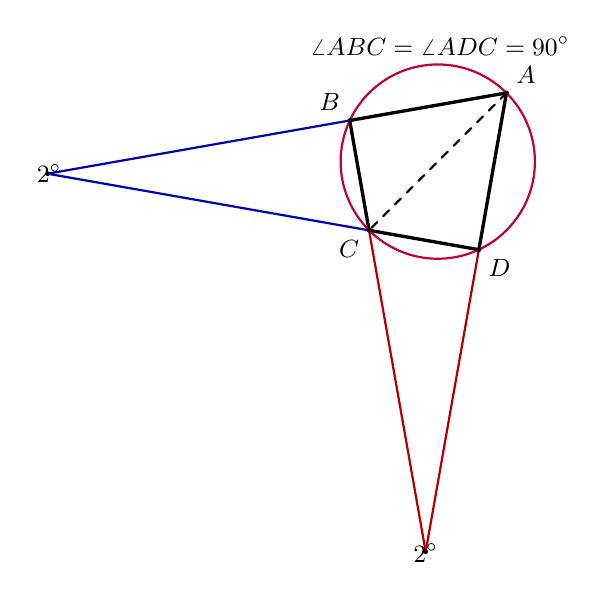
\begin{tikzpicture}[
        scale=1.2,
        line cap=round,
        line join=round,
        every node/.style={font=\small}
    ]

        % 两个测向点
        \coordinate (S1) at (-4,0);
        \coordinate (S2) at (0,-4);

        % 交会四边形的四个顶点
        \coordinate (A) at (0.855,0.855);
        \coordinate (B) at (-0.804,0.563);
        \coordinate (C) at (-0.599,-0.599);
        \coordinate (D) at (0.563,-0.804);

        % AC 中点，即圆心
        \coordinate (O) at ($(A)!0.5!(C)$);

        % 两个 2° 角域
        \fill[blue!10]
            (S1) -- (A) -- (B) -- cycle;
        \fill[red!10]
            (S1) -- (C) -- (D) -- cycle;

        \fill[green!10]
            (S2) -- (B) -- (C) -- cycle;
        \fill[orange!10]
            (S2) -- (D) -- (A) -- cycle;

        % 四条角域边界线
        \draw[blue!70!black,thick] (S1) -- (A);
        \draw[blue!70!black,thick] (S1) -- (D);

        \draw[red!70!black,thick] (S2) -- (B);
        \draw[red!70!black,thick] (S2) -- (A);

        % 交会四边形 ABCD
        \draw[black,very thick]
            (A) -- (B) -- (C) -- (D) -- cycle;

        % 连接 AC
        \draw[black,thick,dashed] (A) -- (C);

        % 以 AC 为直径的圆
        \draw[purple,thick] (O) circle[radius=1.028];

        % 直角标记
        \pic[
            draw,
            angle radius=0.13,
            angle eccentricity=1.2
        ] {right angle=A--B--C};

        \pic[
            draw,
            angle radius=0.13,
            angle eccentricity=1.2
        ] {right angle=A--D--C};

        % 两个角域的角度标记
        \pic[
            draw=blue!70!black,
            "$2^\circ$",
            angle radius=0.42,
            angle eccentricity=1.35
        ] {angle=D--S1--A};

        \pic[
            draw=red!70!black,
            "$2^\circ$",
            angle radius=0.42,
            angle eccentricity=1.35
        ] {angle=B--S2--A};

        % 顶点与测向点
        \fill (A) circle (0.025) node[above right] {$A$};
        \fill (B) circle (0.025) node[above left]  {$B$};
        \fill (C) circle (0.025) node[below left]  {$C$};
        \fill (D) circle (0.025) node[below right] {$D$};

        \fill (S1) circle (0.025);
        \fill (S2) circle (0.025);

        % 直角关系说明
        \node at (0.15,1.35)
            {$\angle ABC=\angle ADC=90^\circ$};

    \end{tikzpicture}

    \caption{$90^\circ$ 特殊构型几何证明示意图}
    \label{fig:90-degree-configuration}
\end{figure}
设两次测向的中心方向夹角为 $\varphi=90^\circ$，测向误差均为 $\pm1^\circ$。由于两组角域中对应边界线之间的夹角仍为 $90^\circ$，其交会形成的凸四边形 $ABCD$ 满足
\[
\angle ABC=\angle ADC=90^\circ.
\]

根据泰勒斯定理的逆定理，点 $B$ 和 $D$ 均位于以 $AC$ 为直径的圆上，因此四边形的四个顶点均位于该圆周上。由于 $AC$ 是圆的直径，也是圆内任意两点间的最大距离，故 $AC$ 同时为该定位四边形的直径。

又因为圆盘为凸集，而定位区域是由四个顶点构成的凸四边形，所以整个定位区域均包含在该圆盘内。因此，当
\[
\varphi=90^\circ
\]
时，以定位区域直径为直径所作的圆一定能够完全覆盖该定位区域。

\subsubsection{临界夹角下的全位置网格验证}
在确定不可覆盖情况主要集中于
\[
\varphi\in(88^\circ,90^\circ)\cup(90^\circ,92^\circ)
\]
后，进一步将夹角固定在上述临界范围内，并对第二监测点的位置进行更高精度的遍历。为减小位置离散化对结果的影响，将位置网格步长由原来的 $100\,\mathrm{m}$ 缩小至
\(10\,\mathrm{m}\)。


在这一更精细的位置网格下，对所有候选位置重新进行覆盖性检验。结果表明，在当前 $10\,\mathrm{m}$ 的位置步长和既定角度精度下，临界夹角范围内的各位置采样点均能产生不可覆盖构型。这说明该现象并非由少数特殊位置导致，而是在临界夹角范围内具有较强的位置普遍性。因此，在当前数值精度下，定位区域的覆盖性主要受两次测向中心方向相对夹角的影响，而对第二监测点具体位置的敏感性相对较弱。












%%%%%%%%%%%%%%%%%%%%%%%%%%%%%%%%%%%%%%%%%%%%%%%%%%%%%%%%%%%%% 
\section{问题二的模型的建立和求解}
\subsection{具体分析}
已知第一监测点的位置及其测得的示向度后，需要进一步确定第二监测点的位置，使两次测向得到的交会定位效果尽可能好。本文将“较优”定义为：假设干扰源在第一监测点示向度对应的射线上等概率分布，当第二监测点选在某一位置时，由两个监测点形成的交会定位区域满足“直径小于 40 m”且“待定检测点与已知检测点检测范围构成的三角形的最远距离不超过1000米"。这样机器狗可直接移动至定位区域附近，并利用光学设备完成进一步探测与清除。

为了将这一概率转化为可计算指标，本文建立第二监测点的几何评分模型。对于任意一个候选第二监测点，沿第一监测点的示向射线考察干扰源可能处于的不同位置，并逐一判断对应交会区域是否同时满足上述两个条件。满足条件的目标数即为得分。因此得分越高，说明该位置作为第二监测点越优。

最后，对平面内各候选监测点进行评分，并选取得分位于前 \(10\%\) 的点，其形成的区域作为第二监测点的较优候选区域。

\subsection{模型准备与候选区域确定}
为便于后续分析，首先对坐标系进行归一化。设第一监测点为
\[
S_1=(0,0),
\]
并令其示向中心线沿 $y$ 轴正方向。由于检测范围及后续约束关于该中心线对称，因此只需计算 $x\geq 0$ 一侧的候选位置，另一侧的结果可通过关于 $y$ 轴镜像得到。

设单次测向的角度误差为 $\varepsilon$，检测距离为
\[
L=1500\,\mathrm{m}.
\]
对于任意监测点 $S$，当其示向度为 $\theta$ 时，检测范围可表示为一个等腰三角形，其三个顶点分别为
\[
V_0=S,
\]
\[
V_1=S+L
\bigl(
\cos(\theta-\varepsilon),
\sin(\theta-\varepsilon)
\bigr),
\]
\[
V_2=S+L
\bigl(
\cos(\theta+\varepsilon),
\sin(\theta+\varepsilon)
\bigr).
\]

记第一监测点的检测区域为 $T_1$。题目要求第二监测点 $S_2$ 到区域 $T_1$ 内任意一点的距离均不超过 $1000\,\mathrm{m}$。由于 $T_1$ 为凸三角形，点到该区域的最远距离可在其顶点处取得，故该约束等价于
\[
\|S_2-V_i\|\leq 1000\,\mathrm{m},
\qquad i=0,1,2.
\]

因此，第二监测点的可选范围可表示为
\[
\Omega
=
\bigcap_{i=0}^{2}
\left\{
P\in\mathbb{R}^2:
\|P-V_i\|\leq 1000\,\mathrm{m}
\right\},
\]
即分别以 $T_1$ 的三个顶点 $V_0,V_1,V_2$ 为圆心、以 $1000\,\mathrm{m}$ 为半径的三个圆盘的公共交集。结合检测区域的对称性，只需在 $\Omega$ 的一侧进行候选点搜索，另一侧可由镜像对称关系直接获得，从而确定后续评分模型所需的第二监测点候选区域。

\subsection{干扰源位置枚举}
假设干扰源在第一监测点的检测区域内均匀分布。由于测向误差角 $\varepsilon$ 较小，可将二维扇形区域近似压缩至中心示向射线上。在归一化坐标系下，第 $i$ 个干扰源的位置记为
\[
G_i=(0,r_i).
\]

对于半径为 $r$、径向宽度为 $\mathrm{d}r$ 的窄扇环，其面积满足
\[
\mathrm{d}A\propto r\,\mathrm{d}r,
\]
因此，二维均匀分布所对应的径向概率密度与 $r$ 成正比。为使各离散枚举点具有近似相同的概率权重，对 $r^2$ 进行等间隔划分，即
\[
r_i=
\sqrt{
r_{\min}^{\,2}
+
\frac{i}{N}
\left(
L^2-r_{\min}^{\,2}
\right)
},
\qquad i=1,2,\ldots,N.
\]

其中，
\[
r_{\min}=30\,\mathrm{m},
\qquad
L=1500\,\mathrm{m},
\qquad
N=150.
\]
通过上述非等距采样方法，可以在一维简化后近似保留原二维均匀分布的概率特征。
\subsection{待定监测点网格枚举}
在约束范围内，仅对 $x\geq 0$ 一侧进行网格搜索。以 $10\,\mathrm{m}$ 为步长进行位置枚举，共得到 $2224$ 个第二监测点候选位置。

对于每个候选位置
\[
S_2=(x_2,y_2),
\]
令其中心检测方向指向第 $i$ 个目标点
\[
G_i=(x_{G_i},y_{G_i}),
\]
则第二监测点的示向角为
\[
\theta_2
=
\operatorname{atan2}
\left(
y_{G_i}-y_2,\,
x_{G_i}-x_2
\right).
\]

由于 $G_i=(0,r_i)$，上式可以进一步写为
\[
\theta_2
=
\operatorname{atan2}
\left(
r_i-y_2,\,
-x_2
\right).
\]
\subsection{优度评定}

对于每个第二监测点候选位置 $S_2$，遍历所有目标点
\[
G_i,\qquad i=1,2,\ldots,N,
\]
并按照以下步骤进行评价：

\begin{enumerate}
    \item 构造第一监测点对应的检测三角形 $T_1$，以及第二监测点朝向目标点 $G_i$ 时对应的检测三角形 $T_{2,i}$；
    
    \item 采用第一问所建立的算法，计算两个检测三角形交会区域的多边形顶点及其直径 $d_i$；
    
    \item 若交会区域的直径满足
    \[
    0<d_i\leq 40\,\mathrm{m},
    \]
    则将该候选位置的有效目标计数加 $1$。
\end{enumerate}

定义候选位置 $S_2$ 的优度分数为交会区域直径不超过 $40\,\mathrm{m}$ 的目标点数量，即
\[
\operatorname{Score}(S_2)
=
\sum_{i=1}^{N}
\mathbf{1}\!\left(0<d_i\leq40\,\mathrm{m}\right),
\]
其中，$\mathbf{1}(\cdot)$ 为示性函数：当括号内条件成立时取值为 $1$，否则取值为 $0$。因此，$\operatorname{Score}(S_2)$ 越大，说明该候选位置能够对越多的目标点实现直径不超过 $40\,\mathrm{m}$ 的定位。


\subsection{模型求解}
\subsubsection{总体分析}
\begin{table}[htbp]
    \centering
    \caption{第二监测点位置搜索结果}
    \label{tab:monitoring-position-results}
    \begin{tabular}{cc}
        \hline
        指标 & 结果 \\
        \hline
        最优检测位置数 & $0$ \\
        良好检测位置数 & $876$ \\
        左右分布 & 左右各 $438$ 个 \\
        纵向范围 & $y\in[500,900]\,\mathrm{m}$ \\
        横向范围 &
        $x\in[-760,-220]\cup[220,760]\,\mathrm{m}$ \\
        总体特征 & 关于 $y$ 轴对称，形成两块高分区域 \\
        \hline
    \end{tabular}
\end{table}


首先，在本次参数设置下，不存在满分候选点，即不存在对所有枚举目标位置都能使交会定位区域直径不超过 $40\,\mathrm{m}$ 的第二监测点。

进一步地，按照“得分位于前 $10\%$”的标准，共筛选出 876 个良好检测位置。这些点在平面上呈现出明显的左右对称分布，说明第二监测点的优良区域主要由几何关系决定，并与第一监测点方向线关于 $y$ 轴对称。

从空间分布上看，良好检测位置整体形状近似为左右对称的椭圆状或纺锤状区域。其纵向分布大致位于
\[
y\in[500,900]\,\mathrm{m},
\]
横向分布大致位于
\[
x\in[-760,-220]\cup[220,760]\,\mathrm{m}.
\]
这表明，较优的第二监测点既不能离第一监测点方向线过近，也不能偏离过远，而是集中在方向线两侧一定距离范围内。

\subsubsection{最优检测位置}

本次计算结果中，最优检测位置数量为 0。

这一结果说明，第二监测点的选择本质上是一个折中优化问题。由于目标可能出现在第一监测射线上的不同位置，而不同位置对应的最佳交会几何关系并不完全一致，因此难以找到对全部目标位置都同时最优的单一点。

\subsubsection{良好检测位置分析}

从图形分布来看，良好检测位置并不是随机散布的，而是形成了两个稳定的高质量区域。

进一步分析可知：

\begin{enumerate}
    \item 过于靠近方向线的位置效果较差。

    若第二监测点过于接近 $y$ 轴，则两次测向形成的夹角偏小，交会区域会被拉长，不利于缩小定位区域直径。

    \item 过远的位置同样不理想。

    若第二监测点离方向线过远，虽然交会角度增大，但对远处目标的几何约束未必稳定，也会降低整体评分。

    \item 中等偏侧的位置更优。

    图中两侧绿色区域说明，当第二监测点位于方向线两侧，并保持适中的横向距离和前向距离时，两次测向形成的交会效果较好，能够兼顾不同目标位置下的定位精度。
\end{enumerate}

因此，从模型输出的角度看，可以将这两片对称区域视为第二监测点的推荐布设区域。


























\newpage
%%%%%%%%%%%%%%%%%%%%%%%%%%%%%%%%%%%%%%%%%%%%%%%%%%%%%%%%%%%%% 
\section{问题三的模型的建立和求解}
\subsection{具体分析}
在完成交会定位区域分析和第二检测点选择策略后，进一步将上述结论应用于更复杂的多干扰源搜索与清除问题。以任务总时间最短为优化目标，总耗时主要由\textbf{定位时间、移动时间和清除时间}组成。因此，问题可转化为：如何合理规划机器狗的动作顺序与运动路径，在保证所有干扰源均被清除的前提下，尽可能降低上述三部分耗时。

由于一次扫描无法覆盖整个目标区域，机器狗需要在不同位置进行多次扫描，因此扫描时机和扫描位置本身就是路径优化的重要部分。对于已经发现的干扰源，为了获得较准确的位置，通常还需要进行第二次测向。根据第二问的结果，可以提前确定较优的第二检测区域，这既有助于缩短移动路程，也能提高一次定位成功的概率，从而减少后续扫描次数和检测时间。

如果两次测向后的交会区域仍然较大，则需要继续补测。是否进行第三次扫描，可以根据第一问得到的定位区域大小和形状进行判断，相应的补测位置同样会影响后续路程。

因此，机器狗在运行过程中实际上需要不断在继续扫描、移动到其他任务点以及前往目标进行光学定位和清除之间作出选择。综合上述因素，本文采用\textbf{基于滚动时域的在线动态重规划策略}：优先处理中心区域内距离较近的任务，并在移动过程中完成沿途的外围扫描与清除；每获得一次新的测量结果或清除结果，便立即更新当前信息并重新规划下一步。该策略既能保证搜索区域得到完整覆盖，又能尽可能减少大范围折返。由于机器狗的移动时间在总任务时间中占比较大，因此\textbf{路径长度是整个策略中最重要的优化对象}。
\subsection{总体策略}
为了利用半径为 $1000\,\mathrm{m}$ 的扫描区域覆盖半径为 $1800\,\mathrm{m}$ 的目标区域，机器狗必须在不同位置进行多次扫描。若在任务开始时单独规划区域覆盖路径，将产生较大的额外移动代价。因此，本文不将区域覆盖与目标清除分开处理，而是将扫描任务与后续的定位、清除任务相融合，尽量利用已有移动路径完成新区域的覆盖。

基于上述思路，本文比较了两种搜索策略。第一种为\textbf{由内向外的滚动覆盖策略}：首先处理内圈目标；当机器狗在定位或清除过程中进入靠近外圈的扫描区域时，利用当前位置完成外围扫描，并继续处理外圈目标。第二种为\textbf{外围优先覆盖策略}：任务开始后直接前往外圈，通过多个扫描点的重叠实现目标区域的完整覆盖，同时就近清除已经发现的目标。

测试结果表明，第一种策略的总用时明显更短。结合运行日志可知，其优势主要来源于对大范围折返的有效减少。由于任务点会随着新测量结果的获得而不断更新，第一种策略在滚动重规划过程中会自然形成近似由内向外扩展的螺旋式路径，使径向移动与扫描、定位及清除任务尽可能重合。虽然该路径在局部上存在一定绕行，但由于能够在同一段移动过程中完成多个任务，因此其整体移动距离和总任务时间反而更小。


\begin{figure}[htbp]
    \centering

    %==================================================
    % 左图：由内向外滚动覆盖策略
    %==================================================
    \begin{subfigure}[t]{0.49\textwidth}
        \centering
        \begin{tikzpicture}
            \begin{axis}[
                width=\linewidth,
                height=1.02\linewidth,
                axis equal image,
                xmin=-2000,
                xmax=1800,
                ymin=-2050,
                ymax=1900,
                xlabel={$x/\mathrm{m}$},
                ylabel={$y/\mathrm{m}$},
                grid=both,
                major grid style={
                    dashed,
                    gray!40,
                    line width=0.25pt
                },
                axis lines=middle,
                tick label style={font=\tiny},
                label style={font=\scriptsize},
                clip=false,
                legend style={
                    font=\tiny,
                    at={(0.5,-0.16)},
                    anchor=north,
                    legend columns=2,
                    draw=gray!50,
                    fill=white,
                    row sep=-1pt
                }
            ]

            % 运动轨迹
            \addplot[
                pathgray,
                line width=0.65pt,
                postaction={decorate},
                decoration={
                    markings,
                    mark=between positions 0.03 and 0.98 step 0.05 with {
                        \arrow{Stealth}
                    }
                },
                forget plot
            ] coordinates {
                (0,0)
                (-422,-335)
                (-86,-532)
                (275,-463)
                (72,-463)
                (359,-868)
                (224,-1000)
                (-94,-1157)
                (692,-1291)
                (1161,-1331)
                (-153,-1582)
                (-359,-868)
                (-460,-804)
                (-868,-359)
                (-1060,144)
                (-1473,297)
                (-1199,761)
                (-1339,1163)
                (-1336,1145)
                (-359,868)
                (-122,524)
                (32,538)
                (338,419)
                (483,237)
                (538,16)
                (695,-255)
                (868,-359)
                (868,359)
                (1226,761)
                (1115,1040)
                (706,782)
                (694,756)
                (688,743)
                (359,868)
                (241,781)
                (313,973)
                (171,1116)
                (155,1075)
                (-329,991)
                (-348,1017)
                (-798,1180)
                (-466,1033)
            };

            % 运动轨迹图例
            \addlegendimage{
                pathgray,
                line width=0.7pt,
                -{Stealth}
            }
            \addlegendentry{运动轨迹}

            % 原点
            \addplot[
                only marks,
                mark=square*,
                mark size=2.5pt,
                startgreen
            ] coordinates {(0,0)};
            \addlegendentry{起点}

            % 第二检测点
            \addplot[
                only marks,
                mark=*,
                mark size=1.7pt,
                detectblue
            ] coordinates {
                (-422,-335)
                (-86,-532)
                (275,-463)
                (-94,-1157)
                (692,-1291)
                (-1060,144)
                (-1199,761)
                (-122,524)
                (32,538)
                (338,419)
                (483,237)
                (538,16)
                (1226,761)
                (-798,1180)
            };
            \addlegendentry{第二检测点}

            % 外围扫描点
            \addplot[
                only marks,
                mark=diamond*,
                mark size=2.3pt,
                scanpurple
            ] coordinates {
                (359,-868)
                (-359,-868)
                (-868,-359)
                (-359,868)
                (868,-359)
                (868,359)
                (359,868)
            };
            \addlegendentry{外围扫描点}

            % 清除未命中点
            \addplot[
                only marks,
                mark=triangle*,
                mark size=2.4pt,
                mark options={
                    draw=missorange,
                    fill=white,
                    line width=0.7pt
                }
            ] coordinates {
                (-1339,1163)
                (706,782)
                (694,756)
                (171,1116)
                (-329,991)
            };
            \addlegendentry{清除未命中}

            % 清除成功点
            \addplot[
                only marks,
                mark=x,
                mark size=2.8pt,
                mark options={
                    clearred,
                    line width=1pt
                }
            ] coordinates {
                (72,-463)
                (224,-1000)
                (1161,-1331)
                (-153,-1582)
                (-460,-804)
                (-1473,297)
                (-1336,1145)
                (695,-255)
                (1115,1040)
                (688,743)
                (241,781)
                (313,973)
                (155,1075)
                (-348,1017)
                (-466,1033)
            };
            \addlegendentry{清除成功}

            % 频道编号
            \node[font=\tiny,clearred,above right]
                at (axis cs:72,-463) {1};
            \node[font=\tiny,clearred,above right]
                at (axis cs:224,-1000) {18};
            \node[font=\tiny,clearred,above right]
                at (axis cs:1161,-1331) {11};
            \node[font=\tiny,clearred,above right]
                at (axis cs:-153,-1582) {6};
            \node[font=\tiny,clearred,above right]
                at (axis cs:-460,-804) {2};
            \node[font=\tiny,clearred,above right]
                at (axis cs:-1473,297) {20};
            \node[font=\tiny,clearred,above right]
                at (axis cs:-1336,1145) {7};
            \node[font=\tiny,clearred,above right]
                at (axis cs:695,-255) {17};
            \node[font=\tiny,clearred,above right]
                at (axis cs:1115,1040) {4};
            \node[font=\tiny,clearred,above right]
                at (axis cs:688,743) {15};
            \node[font=\tiny,clearred,above right]
                at (axis cs:241,781) {3};
            \node[font=\tiny,clearred,above right]
                at (axis cs:313,973) {12};
            \node[font=\tiny,clearred,above right]
                at (axis cs:155,1075) {5};
            \node[font=\tiny,clearred,above right]
                at (axis cs:-348,1017) {19};
            \node[font=\tiny,clearred,above right]
                at (axis cs:-466,1033) {16};

            \end{axis}
        \end{tikzpicture}

        \caption{由内向外滚动覆盖策略}
        \label{fig:inner-outer-route}
    \end{subfigure}
    \hfill
    %==================================================
    % 右图：外围优先覆盖策略
    %==================================================
    \begin{subfigure}[t]{0.49\textwidth}
        \centering
        \begin{tikzpicture}
            \begin{axis}[
                width=\linewidth,
                height=1.02\linewidth,
                axis equal image,
                xmin=-2000,
                xmax=1800,
                ymin=-2050,
                ymax=1900,
                xlabel={$x/\mathrm{m}$},
                ylabel={$y/\mathrm{m}$},
                grid=both,
                major grid style={
                    dashed,
                    gray!40,
                    line width=0.25pt
                },
                axis lines=middle,
                tick label style={font=\tiny},
                label style={font=\scriptsize},
                clip=false,
                legend style={
                    font=\tiny,
                    at={(0.5,-0.16)},
                    anchor=north,
                    legend columns=2,
                    draw=gray!50,
                    fill=white,
                    row sep=-1pt
                }
            ]

            % 半径为1800 m的目标区域边界
            \addplot[
                gray,
                dotted,
                line width=0.6pt,
                domain=0:360,
                samples=180,
                forget plot
            ]
            ({1800*cos(x)},{1800*sin(x)});

            % 运动轨迹
            \addplot[
                pathgray,
                line width=0.65pt,
                postaction={decorate},
                decoration={
                    markings,
                    mark=between positions 0.03 and 0.98 step 0.05 with {
                        \arrow{Stealth}
                    }
                },
                forget plot
            ] coordinates {
                (0,0)
                (0,1000)
                (-270,490)
                (148,811)
                (56,746)
                (782,623)
                (975,-223)
                (1549,-601)
                (1258,-328)
                (1220,-442)
                (434,-901)
                (376,-560)
                (-49,-711)
                (-30,-609)
                (821,-892)
                (698,-932)
                (842,-897)
                (949,-1268)
                (937,-1021)
                (401,-1588)
                (231,-1934)
                (291,-1689)
                (-434,-901)
                (-975,-223)
                (-1008,-523)
                (-1027,-624)
                (-1415,305)
                (-1508,254)
                (-782,623)
                (-1165,438)
                (-1121,822)
                (-1087,587)
                (-1186,654)
                (-1246,830)
                (-1061,936)
                (-1048,1072)
            };

            % 运动轨迹图例
            \addlegendimage{
                pathgray,
                line width=0.7pt,
                -{Stealth}
            }
            \addlegendentry{运动轨迹}

            % 起点
            \addplot[
                only marks,
                mark=square*,
                mark size=2.5pt,
                startgreen
            ] coordinates {(0,0)};
            \addlegendentry{起点}

            % 覆盖圆心
            \addplot[
                only marks,
                mark=diamond*,
                mark size=2.3pt,
                scanpurple
            ] coordinates {
                (0,1000)
                (782,623)
                (975,-223)
                (434,-901)
                (-434,-901)
                (-975,-223)
                (-782,623)
            };
            \addlegendentry{覆盖圆心}

            % 检测点
            \addplot[
                only marks,
                mark=*,
                mark size=1.7pt,
                detectblue
            ] coordinates {
                (0,1000)
                (-270,490)
                (782,623)
                (975,-223)
                (1549,-601)
                (1258,-328)
                (434,-901)
                (376,-560)
                (-49,-711)
                (821,-892)
                (842,-897)
                (949,-1268)
                (401,-1588)
                (231,-1934)
                (-434,-901)
                (-975,-223)
                (-1008,-523)
                (-1415,305)
                (-782,623)
                (-1165,438)
                (-1121,822)
                (-1186,654)
                (-1061,936)
            };
            \addlegendentry{检测点}

            % 清除成功点
            \addplot[
                only marks,
                mark=x,
                mark size=2.8pt,
                mark options={
                    clearred,
                    line width=1pt
                }
            ] coordinates {
                (148,811)
                (56,746)
                (1220,-442)
                (-30,-609)
                (698,-932)
                (937,-1021)
                (291,-1689)
                (-1027,-624)
                (-1508,254)
                (-1087,587)
                (-1246,830)
                (-1048,1072)
            };
            \addlegendentry{清除成功}

            % 频道编号
            \node[font=\tiny,clearred,above right]
                at (axis cs:148,811) {19};
            \node[font=\tiny,clearred,above right]
                at (axis cs:56,746) {11};
            \node[font=\tiny,clearred,above right]
                at (axis cs:1220,-442) {6};
            \node[font=\tiny,clearred,above right]
                at (axis cs:-30,-609) {5};
            \node[font=\tiny,clearred,above right]
                at (axis cs:698,-932) {10};
            \node[font=\tiny,clearred,above right]
                at (axis cs:937,-1021) {12};
            \node[font=\tiny,clearred,above right]
                at (axis cs:291,-1689) {15};
            \node[font=\tiny,clearred,above right]
                at (axis cs:-1027,-624) {20};
            \node[font=\tiny,clearred,above right]
                at (axis cs:-1508,254) {17};
            \node[font=\tiny,clearred,above right]
                at (axis cs:-1087,587) {3};
            \node[font=\tiny,clearred,above right]
                at (axis cs:-1246,830) {9};
            \node[font=\tiny,clearred,above right]
                at (axis cs:-1048,1072) {7};

            \end{axis}
        \end{tikzpicture}

        \caption{外围优先覆盖策略}
        \label{fig:outer-first-route}
    \end{subfigure}

    \caption{两种机器狗搜索与清除策略的运动轨迹对比}
    \label{fig:route-comparison}
\end{figure}




\subsection{优化方式}
\subsubsection{扫描优化}
对于任一干扰源，通常至少需要进行两次测向，才能将其位置缩小至可进行光学定位和清除的范围。本文将用于发现目标的全频道扫描记为\textbf{A 类扫描}，将针对已发现目标进行的补充测向记为\textbf{B 类扫描}。

若干扰源位于机器狗当前扫描点半径为 $1000\,\mathrm{m}$ 的有效探测范围内，则可在相应的 A 类扫描中获得第一次示向度。\textbf{内圈目标}通常在\textbf{原点的首次扫描中被发现}，外圈目标则在机器狗后续进入外圈或外围扫描点时被发现。对于尚未发现目标的频道，在后续 A 类扫描中继续进行检测，直至该频道被发现，或其可能存在的区域已被扫描范围完全覆盖。

获得第一次示向度后，调用第二问的计算结果确定较优的第二监测区域，并从中选择具体位置作为\textbf{第二监测点}进行 B 类扫描。
方法如下：
第一次 A 类扫描得到示向度后，根据第二问确定第二检测点的较优区域 \(\Omega_{\mathrm{good}}\)。以第一次检测点 \(S_1\) 和示向角 \(\theta\) 建立局部坐标系，对任一候选点 \(P\)，定义前向距离和横向偏移为

$$ d_f=(P-S_1)\cdot(\cos\theta,\sin\theta), $$ $$ d_l=(P-S_1)\cdot(-\sin\theta,\cos\theta). $$

为保证交会几何条件，保留满足

$$ 500\le d_f\le 900,\qquad |d_l|\ge 200 $$

的候选点，即第二监测点既沿示向方向适当前进，又与原示向线保持一定横向距离，避免两次测向近似共线。

随后在这些候选点中综合考虑移动距离和预测定位精度，构造评分函数

$$ J(P)=d(P,P_{\mathrm{cur}})+\alpha D_{\mathrm{pred}}(P)+\beta d(P,G_{\mathrm{nom}}), $$

最终取

$$ P^*=\arg\min J(P) $$

作为实际第二监测点。这样既保证了较好的交会定位效果，也兼顾了后续移动路程。

完成第二次测向后，利用交会定位法计算定位区域，并将其直径记为 $D$。根据 $D$ 的大小，采取如下处理策略：
\[
\begin{cases}
D\leq 40\,\mathrm{m}, 
& \text{直接进入光学定位与清除阶段；}\\[2mm]
40\,\mathrm{m}<D\leq 300\,\mathrm{m},
& \text{先前往直径圆圆心尝试光学定位；}\\[2mm]
D>300\,\mathrm{m},
& \text{直接前往直径圆圆心进行B类扫描。}
\end{cases}
\]

当 $D\leq 40\,\mathrm{m}$ 且以区域直径为直径的圆能够覆盖整个定位区域时，该圆半径不超过 $20\,\mathrm{m}$。因此，机器狗前往直径圆圆心后，即可满足光学探测范围要求。程序相应地将 $40\,\mathrm{m}$ 设置为精确定位阈值。

对于 $40\,\mathrm{m}<D\leq 300\,\mathrm{m}$ 的情况，机器狗首先前往当前估计位置尝试进行光学定位。若能够发现目标，则直接完成清除；若未发现目标，则在当前位置进行一次新的 B 类扫描，并将新获得的示向度与此前的测量结果共同用于交会定位，从而进一步缩小目标的可行区域。

为了完成\textbf{外圈的 A 类扫描}，本文设置了\textbf{黄区覆盖策略}，在保证不遗漏干扰源的同时，尽可能减少专程扫描所产生的额外移动路程。

由于干扰源有效接收半径的下界为 $1000\,\mathrm{m}$，只要检测点与干扰源之间的距离不超过 $1000\,\mathrm{m}$，机器狗就一定能够接收到相应信号。为了覆盖半径为 $1800\,\mathrm{m}$ 的整个目标区域，本文在半径约为 $939\,\mathrm{m}$ 的圆周上设置 $8$ 个扫描中点，其极角分别为
\[
\theta_k
=
22.5^\circ+45^\circ k,
\qquad
k=0,1,\ldots,7.
\]

扫描中点所在圆周的半径由下式确定：
\[
a^2
-2\times1800\cos 22.5^\circ\cdot a
+\left(1800^2-1000^2\right)
=0.
\]
取该方程的较小正根，得到
\[
a\approx938.06\,\mathrm{m}.
\]
实际计算时，将扫描中点半径近似取为
\[
a\approx939\,\mathrm{m}.
\]

原点与上述 $8$ 个扫描中点分别作为扫描圆的圆心，各扫描圆半径均为 $1000\,\mathrm{m}$。这些扫描圆的并集能够覆盖半径为 $1800\,\mathrm{m}$ 的整个目标区域，从而保证搜索过程中不发生漏检。

在实际执行过程中，这 $8$ 个扫描中点首先作为备用扫描航点加入动态任务池。如果机器狗在执行 B/C 类补充测向或清除任务时已经进入
\[
r\geq700\,\mathrm{m}
\]
的外围区域，并且在当前位置执行扫描能够补全某个尚未覆盖的扇区，则机器狗直接在当前位置完成 A 类扫描，同时跳过该扇区对应的备用扫描中点。通过这种处理，可以将全局覆盖过程尽可能融入原有的定位与清除路径中，从而减少为完成外围扫描而产生的额外移动。

扇区覆盖状态采用离散采样方法进行判定。对于每个扇区，分别选取 $5$ 个径向采样位置和 $5$ 个角度采样位置，共得到
\[
5\times5=25
\]
个采样点。只有当该扇区内的全部采样点均落入已有扫描点的 $1000\,\mathrm{m}$ 探测范围内时，才判定该扇区已经完成覆盖。






\subsubsection{任务选择优化}

机器狗当前需要执行的任务可以统一划分为三类：A 类扫描、B/C 类补充测向，以及光学定位与清除。每完成一次任务，系统的当前状态都会随之更新，并可能产生新的待执行任务。因此，整个过程可以视为一个\textbf{动态任务集上的在线路径规划问题}。

具体而言，完成 A 类扫描后，部分频道会被标记为已发现，并根据第二问的计算结果生成相应的 B 类扫描航点；完成 B 类扫描后，根据交会定位区域的大小，可能生成光学定位与清除任务，也可能继续生成新的补测任务。当机器狗在执行 B/C 类扫描或清除任务的过程中进入外围扫描区域时，还可能触发新的 A 类扫描。因此，任务集合会随探测结果不断变化，可表示为
\[
\mathcal{T}_{k+1}
=
F\left(\mathcal{T}_k,s_k\right),
\]
其中，$\mathcal{T}_k$ 表示第 $k$ 次决策时的待执行任务集，$s_k$ 表示本次扫描或清除所获得的新信息。

由于扫描次数已经通过前述定位策略得到尽可能的压缩，而单次检测时间和清除时间基本固定，因此后续最主要的优化空间集中在机器狗的移动距离上。本文将当前所有待执行任务统一视为航点，并以总路径长度最短为主要优化目标：
\[
\min L
=
\sum_{i=0}^{n-1}
d\left(P_i,P_{i+1}\right),
\]
其中，$P_i$ 表示机器狗访问的第 $i$ 个航点，$d(P_i,P_{i+1})$ 表示相邻航点之间的欧氏距离。

具体采用\textbf{最近邻与 2-opt 相结合的在线滚动重规划策略}。首先从机器狗当前位置出发，利用最近邻贪心算法生成一条初始路径，即每次优先选择距离当前位置最近的未完成航点；随后采用 2-opt 算法对初始路径进行局部边交换，以减少路径交叉和不必要的折返。

程序并不一次执行完整的规划路径，而是仅执行当前规划结果中的下一个航点。完成该任务后，根据新获得的测量信息或清除结果更新任务集合，并重新规划下一步。具体而言，程序将第二检测点、补充测向点、清除点和外围扫描点统一加入航点池，再通过最近邻和 2-opt 算法进行在线重规划。

本文没有采用经典动态规划方法。这是因为待执行任务的数量和位置会随着机器狗的运行不断变化，难以在任务开始时预先获得完整且固定的状态空间。相比之下，滚动式启发算法能够根据实时获得的信息快速更新路线，更适合本问题的在线决策场景。程序中的路径规划函数同样先利用最近邻算法构造初始访问顺序，再通过 2-opt 进行局部优化，从而在较低计算复杂度下获得较短的运动路径。

\subsubsection{简单容错机制}
程序还设置了简单的容错机制，以避免单次测量异常导致任务中断。具体处理方式如下：

\begin{enumerate}
    \item 当检测结果为 \texttt{near} 时，表示机器狗与干扰源的距离不超过 $5\,\mathrm{m}$。此时直接在当前位置执行清除；若清除失败，则在周围半径为 $40\,\mathrm{m}$ 的圆周上沿 $8$ 个方向进行搜索，并再次尝试清除。

    \item 当第二检测点返回 \texttt{no\_signal} 时，根据当前估计位置重新选择补测点；若补测次数超过 $6$ 次，则撤销当前定位任务，并将该频道重新交回扫描流程。

    \item 当多次补测后仍无法实现精确定位时，撤销当前在途任务，转向距离目标估计位置最近的黄区扫描点，并在该扫描点重新进行检测。
\end{enumerate}

通过上述容错机制，当出现测量失败、定位结果不稳定或目标距离估计偏差较大等情况时，程序能够自动调整后续任务，无须中断整个搜索与清除过程。

\subsection{模型求解}
\begin{table}[htbp]
    \centering
    \caption{问题3正式测试结果}
    \renewcommand{\arraystretch}{1.6}
    \begin{tabular}{|c|c|c|c|}
        \hline
        测试案例编码 & 清除干扰源个数 & 平均定位清除时间 & 程序运行时间 \\
        \hline
        测试1案例编码 & 11 & 347.5 s/个 & 1.0 s \\
        \hline
        测试2案例编码 & 13 & 300.4 s/个 & 0.9 s \\
        \hline
        测试3案例编码 & 15 & 257.6 s/个 & 0.9 s \\
        \hline
    \end{tabular}
\end{table}

在三次正式测试中，机器狗分别清除了 $11$、$13$ 和 $15$ 个干扰源，平均每个干扰源定位清除时间分别为 $347.5\,\mathrm{s}$、$300.4\,\mathrm{s}$ 和 $257.6\,\mathrm{s}$，对应的定位清除总时间分别为 $3822.7\,\mathrm{s}$、$3904.9\,\mathrm{s}$ 和 $3864.2\,\mathrm{s}$。多次演练及正式测试结果表明，该策略均能完成全部干扰源的搜索与清除，且总任务时间波动较小，未出现明显异常结果，说明该策略具有较好的完整性和稳定性。

随着干扰源数量的增加，平均定位清除时间呈现一定的下降趋势。这可能是因为全区域覆盖所需的外围扫描具有一定的固定开销，而在多目标场景下，不同目标的扫描、补测和清除任务能够共享部分移动路径，使固定开销由更多目标共同分担。同时，任务合并与在线滚动重规划能够减少重复移动和大范围折返，说明本文所采用的路径规划策略具有较好的优化效果。

三次测试的程序运行时间均不超过 $1\,\mathrm{s}$，远小于实际任务执行时间，表明该算法的计算开销较低，能够满足实时决策的需求。













\newpage
%%%%%%%%%%%%%%%%%%%%%%%%%%%%%%%%%%%%%%%%%%%%%%%%%%%%%%%%%%%%% 
\section{问题四的模型的建立和求解}
\subsection{具体分析}

\subsection{模型准备}

\subsection{模型建立}

\subsection{模型求解}



























\newpage
%%%%%%%%%%%%%%%%%%%%%%%%%%%%%%%%%%%%%%%%%%%%%%%%%%%%%%%%%%%%%
\section{模型的评价、改进与推广}

\subsection{模型的优点}
\begin{itemize}[itemindent=2em]
\item 优点1
\item 优点2
\item 优点3
\end{itemize}

\subsection{模型的缺点}
\begin{itemize}[itemindent=2em]
\item 缺点1
\item 缺点2
\end{itemize}




\subsection{模型的改进}






\subsection{模型的推广}






































\newpage
%%%%%%%%%%%%%%%%%%%%%%%%%%%%%%%%%%%%%%%%%%%%%%%%%%%%%%%%%%%%%
%% 参考文献
\nocite{*}
\bibliographystyle{gbt7714-numerical}  % 引用格式
\bibliography{ref.bib}  % bib源














\newpage
%%%%%%%%%%%%%%%%%%%%%%%%%%%%%%%%%%%%%%%%%%%%%%%%%%%%%%%%%%%%%
%% 附录
\begin{appendices}
	
	
	
	
\section{文件列表}
\begin{table}[H]
\centering
\begin{tabularx}{\textwidth}{LL}
\toprule
文件名   & 功能描述 \\
\midrule
%%%%%%%%%%%%%%%%%%%%%%%%%%%%%%%%%%%%%%%%%%%%%%%%%%%%%%%%%%%%%
数据预处理.py & 预处理程序代码 \\
q2.py & 问题二程序代码 \\
q3.c & 问题三程序代码 \\
q4.cpp & 问题四程序代码 \\
%%%%%%%%%%%%%%%%%%%%%%%%%%%%%%%%%%%%%%%%%%%%%%%%%%%%%%%%%%%%%
\bottomrule
\end{tabularx}
\label{tab:文件列表}
\end{table}








%\section{代码}
%\noindent 
%%%%%%%%%%%%%%%%%%%%%%%%%%%%%%%%%%%%%%%%%%%%
%数据预处理.py
%\lstinputlisting[language=python]{code/1.数据预处理.py}
%%%%%%%%%%%%%%%%%%%%%%%%%%%%%%%%%%%%%%%%%%%%%
%
%%%%%%%%%%%%%%%%%%%%%%%%%%%%%%%%%%%%%%%%%%%%
%q2.py
%\lstinputlisting[language=python]{code/q2.py}
%%%%%%%%%%%%%%%%%%%%%%%%%%%%%%%%%%%%%%%%%%%%
%
%
%q3.c
%\lstinputlisting[language=c]{code/q3.c}
%
%
%q4.cpp
%\lstinputlisting[language=c++]{code/q4.cpp}

\end{appendices}
\end{document}
